\documentclass[manuscript,screen]{acmart}
\usepackage{placeins} % for \FloatBarrier

\AtBeginDocument{%
  \providecommand\BibTeX{{%
    \normalfont B\kern-0.5em{\scshape i\kern-0.25em b}\kern-0.8em\TeX}}}

\setcopyright{acmcopyright}
\copyrightyear{2024}
\acmYear{2024}
\acmDOI{XXXXXXX.XXXXXXX}

\begin{document}

\title{Examining Memory Retention Through Rapid Serial Visual Presentation Reading}

\author{Micah Eisele}
\affiliation{%
  \institution{Colorado State University}
  \city{Fort Collins}
  \state{Colorado}
  \country{United States}
}

\renewcommand{\shortauthors}{Eisele}

\begin{abstract}
  This study investigates the efficacy of Rapid Serial Visual Presentation (RSVP) compared to static text methods in enhancing reading comprehension. Utilizing story prompts, four participants were exposed to both RSVP and static text formats, followed by comprehension assessments. Findings suggest a significant difference in comprehension between the two methods, with static text yielding superior retention, however further study is needed due to methodological concerns. Participant feedback highlighted minor issues with screen brightness, underscoring the need for methodological refinement. This research contributes to understanding RSVP's role in education and suggests avenues for future investigation.
\end{abstract}


\begin{CCSXML}
<ccs2012>
   <concept>
       <concept_id>10003120.10003121.10003125.10010591</concept_id>
       <concept_desc>Human-centered computing~Displays and imagers</concept_desc>
       <concept_significance>500</concept_significance>
       </concept>
   <concept>
       <concept_id>10003120.10003121.10003126</concept_id>
       <concept_desc>Human-centered computing~HCI theory, concepts and models</concept_desc>
       <concept_significance>500</concept_significance>
       </concept>
   <concept>
       <concept_id>10003120.10003121.10011748</concept_id>
       <concept_desc>Human-centered computing~Empirical studies in HCI</concept_desc>
       <concept_significance>500</concept_significance>
       </concept>
   <concept>
       <concept_id>10003120.10003121.10003129.10011756</concept_id>
       <concept_desc>Human-centered computing~User interface programming</concept_desc>
       <concept_significance>100</concept_significance>
       </concept>
   <concept>
       <concept_id>10003120.10003121.10003124.10010865</concept_id>
       <concept_desc>Human-centered computing~Graphical user interfaces</concept_desc>
       <concept_significance>100</concept_significance>
       </concept>
   <concept>
       <concept_id>10003120.10003121.10003122.10003334</concept_id>
       <concept_desc>Human-centered computing~User studies</concept_desc>
       <concept_significance>500</concept_significance>
       </concept>
 </ccs2012>
\end{CCSXML}

\ccsdesc[500]{Human-centered computing~Displays and imagers}
\ccsdesc[500]{Human-centered computing~HCI theory, concepts and models}
\ccsdesc[500]{Human-centered computing~Empirical studies in HCI}
\ccsdesc[100]{Human-centered computing~User interface programming}
\ccsdesc[100]{Human-centered computing~Graphical user interfaces}
\ccsdesc[500]{Human-centered computing~User studies}

\keywords{reading, rapid-serial visual presentation, studying, speed reading, memory}

\maketitle

\section{Introduction}
A very large aspect (especially when you get higher up) in education are readings. Typically, at least for colleges, each week a reading is assigned with the intent to supplement the lectures. However, for many, this is a rather daunting task as the process of reading itself takes a long time – with many opting to skip reading entirely leading to lower quiz scores and understanding of the material.

With this in mind, Rapid Serial Visual Presentation (RSVP) reading may be the answer many are looking for. A technique that involves flashing text on a screen, RSVP has been shown to effect reading speed in works like “Crowding and eccentricity determine reading rate” by Pelli et al. [1] where participants were asked to react to letters on a screen with their corresponding button. And it also has been shown to be an effective tool for rifling through long lists of things, like in Spence’s article “Rapid, Serial and Visual: a presentation technique with potential” [2].

This study aims to explore this reading technique, but through a different avenue. Being able to read faster is nice, but retaining that information is crucial. What we attempted to find is whether or not utilizing a form of RSVP that flashes the words individually from a reading significantly affects the reader's understanding of the text in their working memory. Our experiment, which was carried out via four participants, found that the trade-off did indeed exist but the small sample size combined with the small question pool leads room for further inquiry.

\section{Related Works}
\subsection{Reading Rate Improvement Quantified}
There have already been other experiments that have explored RSVP reading. Rubin and Turano's article, "Reading Without Saccadic Eye Movements" [3], measured the reading rates of people using RSVP versus not using RSVP and found that their reading rates improved on average between 2 and 4-fold.

\subsection{Trade-off Using Sentence-based RSVP}
Of course, there have been studies that explored whether there is a significant trade-off between speed and accuracy using RSVP. "So Much to Read, So Little Time: How Do We Read, and Can Speed Reading Help?" by Rayner et al. [4] provides a comprehensive overview of a multitude of studies that have tested whether or not this trade-off exists in speed reading methods in general (with a particular focus in RSVP reading), theorizing that this trade-off does indeed exist based on the information gleaned from the studies analyzed. However, in the sections where they analyzed RSVP, they examined RSVP methods that flashed either one or more sentences as opposed to singular letters.

\begin{table*}[htbp]
  \caption{Prior studies that have analyzed RSVP reading versus traditional methods.}
  \label{tab:freq}
  \tiny
  \begin{tabular}{cccccl}
    \toprule
    \textbf{Paper} & \textbf{Participant Type} & \textbf{Modalities} & \textbf{Delivery Method} & \textbf{Software Tested} & \textbf{Focus/Conclusion} \\
    \midrule
    This paper & Naive users & Desktop Screen & Single Words & Custom & Focused on whether or not an advantage to memory retention is presented when comparing static and\\ &&&&& RSVP text reading methods. Found that static text presents an advantage. \\
    \bottomrule
  \end{tabular}
\end{table*}

\section{Methodology}
\subsection{Prompts.} 
Story prompts were generated using ChatGPT to ensure impartiality and eliminate bias in prompt creation. Each prompt was specifically designed to be comprehensible to the majority of English-speaking adults, requiring no prior knowledge or experience. The prompts were presented in both RSVP and static text formats to compare comprehension and reading speed between the two conditions.

\subsection{Participants.} 
Four native English-speaking individuals, aged between 21 to 59, were recruited for this experiment. Participants had familiarity with desktop computers. However, in order to prevent  any possible legacy bias from occurring, none of the participants chosen had familiarity with RSVP reading methods.

\subsection{Apparatus.} 
A computer program created for this experiment was utilized to present the story prompts and record participant responses. The program automatically centered the text on the screen, which was displayed on a high-resolution monitor with a resolution of $2560 \times 1440$ pixels. Participants used a mouse for input. Before each section, participants received a welcome message shown in Figure 1 and Figure 2 explaining the task (reading a prompt with RSVP or a static method and being quizzed on it after) and underwent a three-second countdown after confirming their readiness. Text was displayed using a white background and black sans-serif font. This is to keep in line with recommendations for a high-contrast background and font for readability from the study, "The impact of web page text-background colour combinations on readability, retention, aesthetics and behavioural intention," by Hall and Hanna [5] and recommendations for sans-serif font to improve readability from the study, "Letter and symbol misrecognition in highly legible typefaces for general, children, dyslexic, visually impaired and ageing readers," by Thomas Bohm [6]. Scores were recorded in a text document automatically indicating participant number and their responses and were not provided to participants to prevent potential bias in their feedback.

\begin{figure}[htbp]
  \centering
  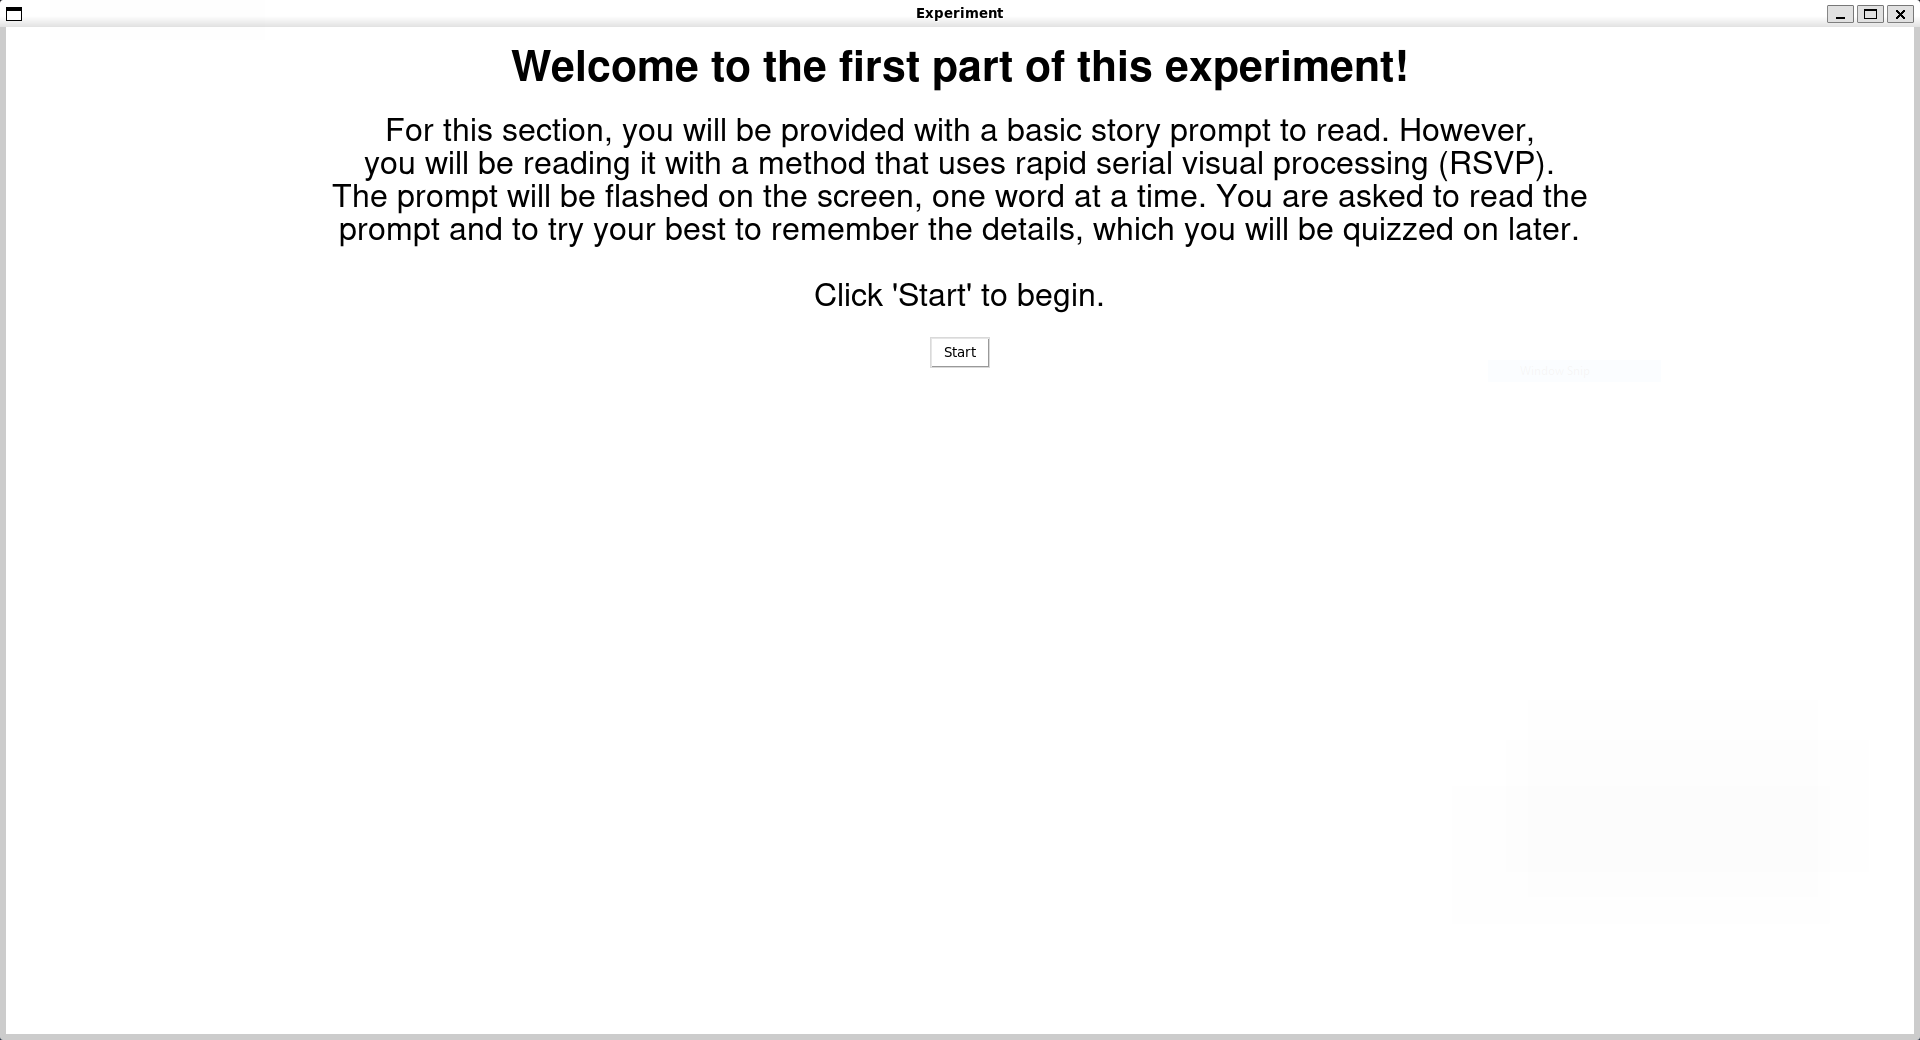
\includegraphics[width=\linewidth]{welcome-rsvp.PNG}
  \caption{The welcome screen for the RSVP text prompt.}
  \Description{"For this section, you will be provided with a basic story prompt to read. However, you will be reading it with a method that uses rapid serial visual processing (RSVP). The prompt will be flashed on the screen, one word at a time. You are asked to read the prompt and to try your best to remember the details, which you will be quizzed on later."}
\end{figure}

\begin{figure}[htbp]
  \centering
  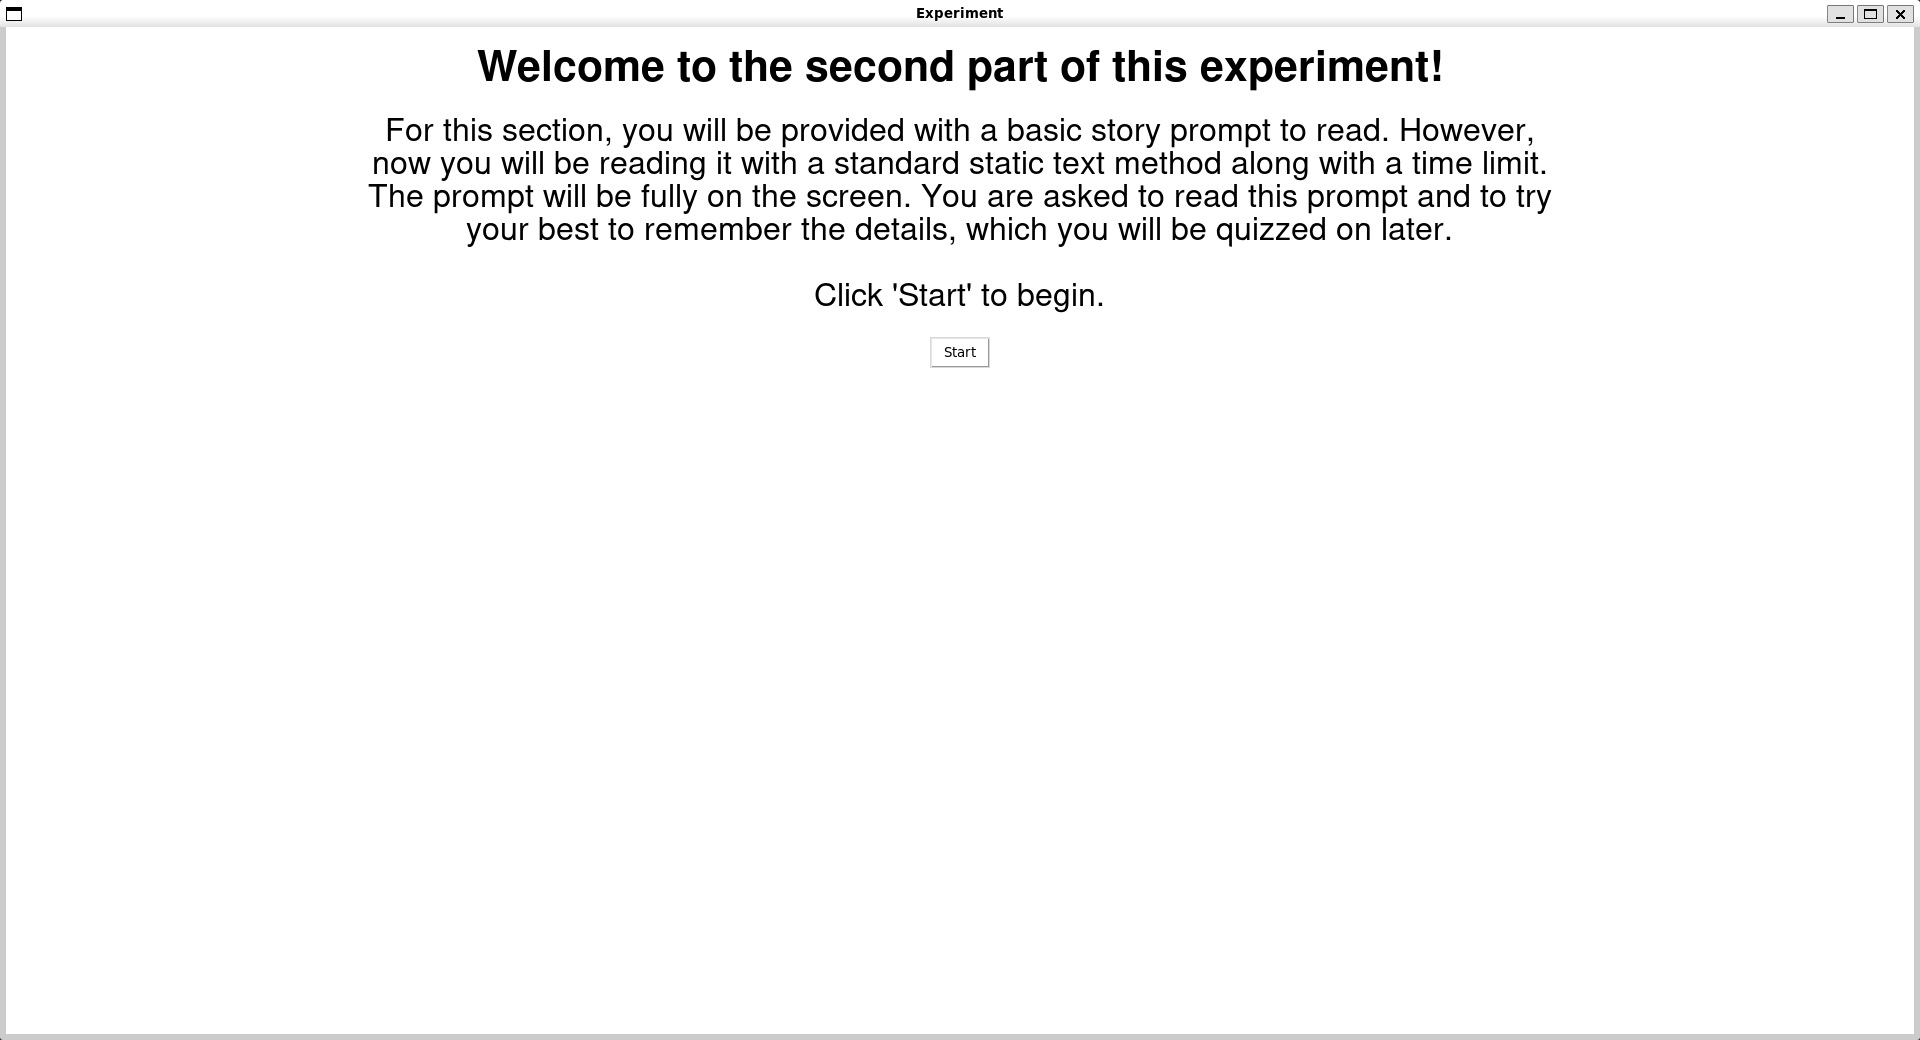
\includegraphics[width=\linewidth]{welcome-static.PNG}
  \caption{The welcome screen for the static text prompt.}
  \Description{"For this section, you will be provided with a basic story prompt to read. However, now you will be reading it with a standard static text method along with a time limit. The prompt will be fully on the screen. You are asked to read this prompt and to try your best to remember the details, which you will be quizzed on later."}
\end{figure}

\FloatBarrier

\subsection{Procedure.} 
Volunteer participants were first briefed on the experiment's procedures. They were then presented with two story prompts of similar difficulty, each assigned to one presentation format: RSVP or static text. For the RSVP section, the text was presented at a speed of 400 words per minute (WPM), maintaining consistency with the low-end of average reading speed increases observed in previous studies (2-fold). For the static text section, participants were given the same prompt but were allotted double the time it would take to assuming a reading rate of 200 WPM chosen on the low-side of the range using the meta-analysis written by Marc Brysbaert, "How many words do we read per minute? A review and meta-analysis of reading rate" [7].

\begin{figure}[htbp]
  \centering
  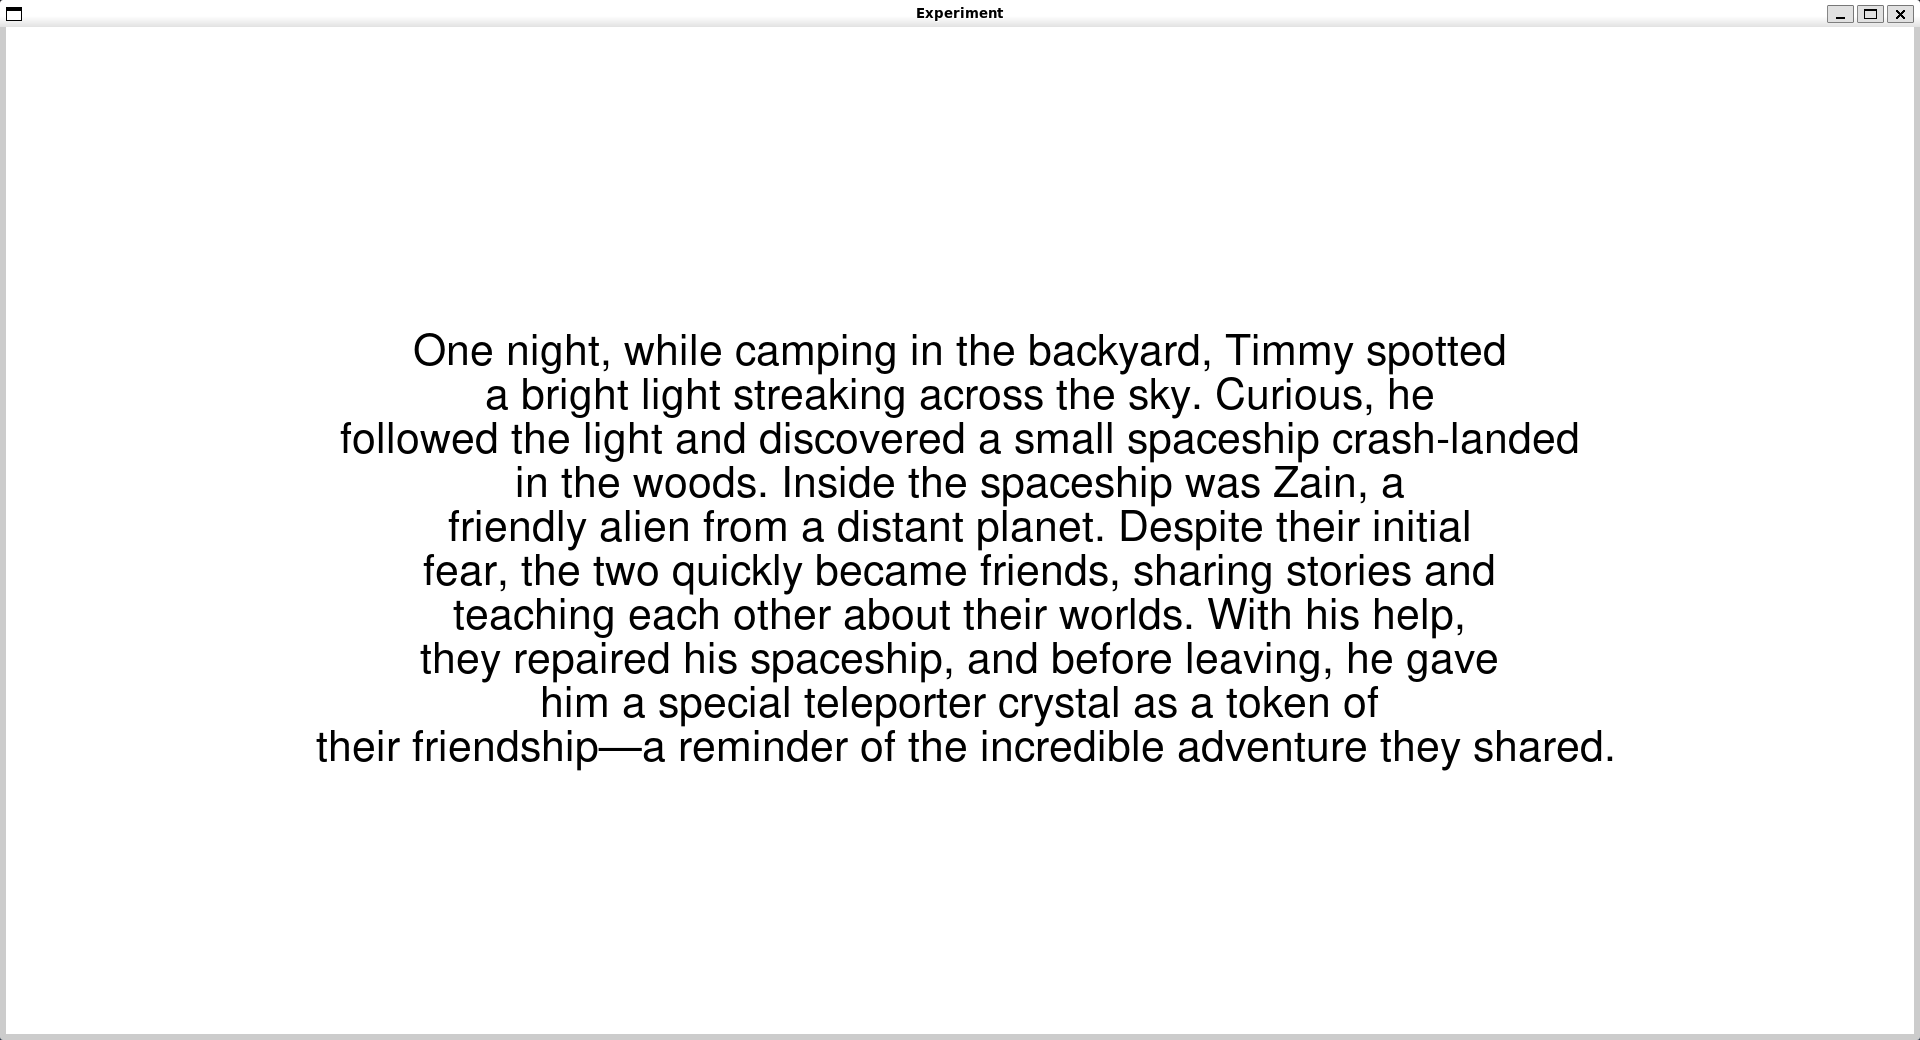
\includegraphics[width=\linewidth]{static-prompt.PNG}
  \caption{The static prompt displayed.}
  \Description{"One night, while camping in the backyard, Timmy spotted a bright light streaking across the sky. Curious, he followed the light and discovered a small spaceship crash-landed in the woods. Inside the spaceship was Zain, a friendly alien from a distant planet. Despite their initial fear, the two quickly became friends, sharing stories and teaching each other about their worlds. With his help, they repaired his spaceship, and before leaving, he gave him a special teleporter crystal as a token of their friendship—a reminder of the incredible adventure they shared."}
\end{figure}

\FloatBarrier

After each section, participants completed a three-question multiple-choice quiz assessing their comprehension of the prompt. Participant responses were recorded electronically by the computer program. Feedback was obtained from participants regarding any difficulties encountered during the task.

\begin{figure}[htbp]
  \centering
  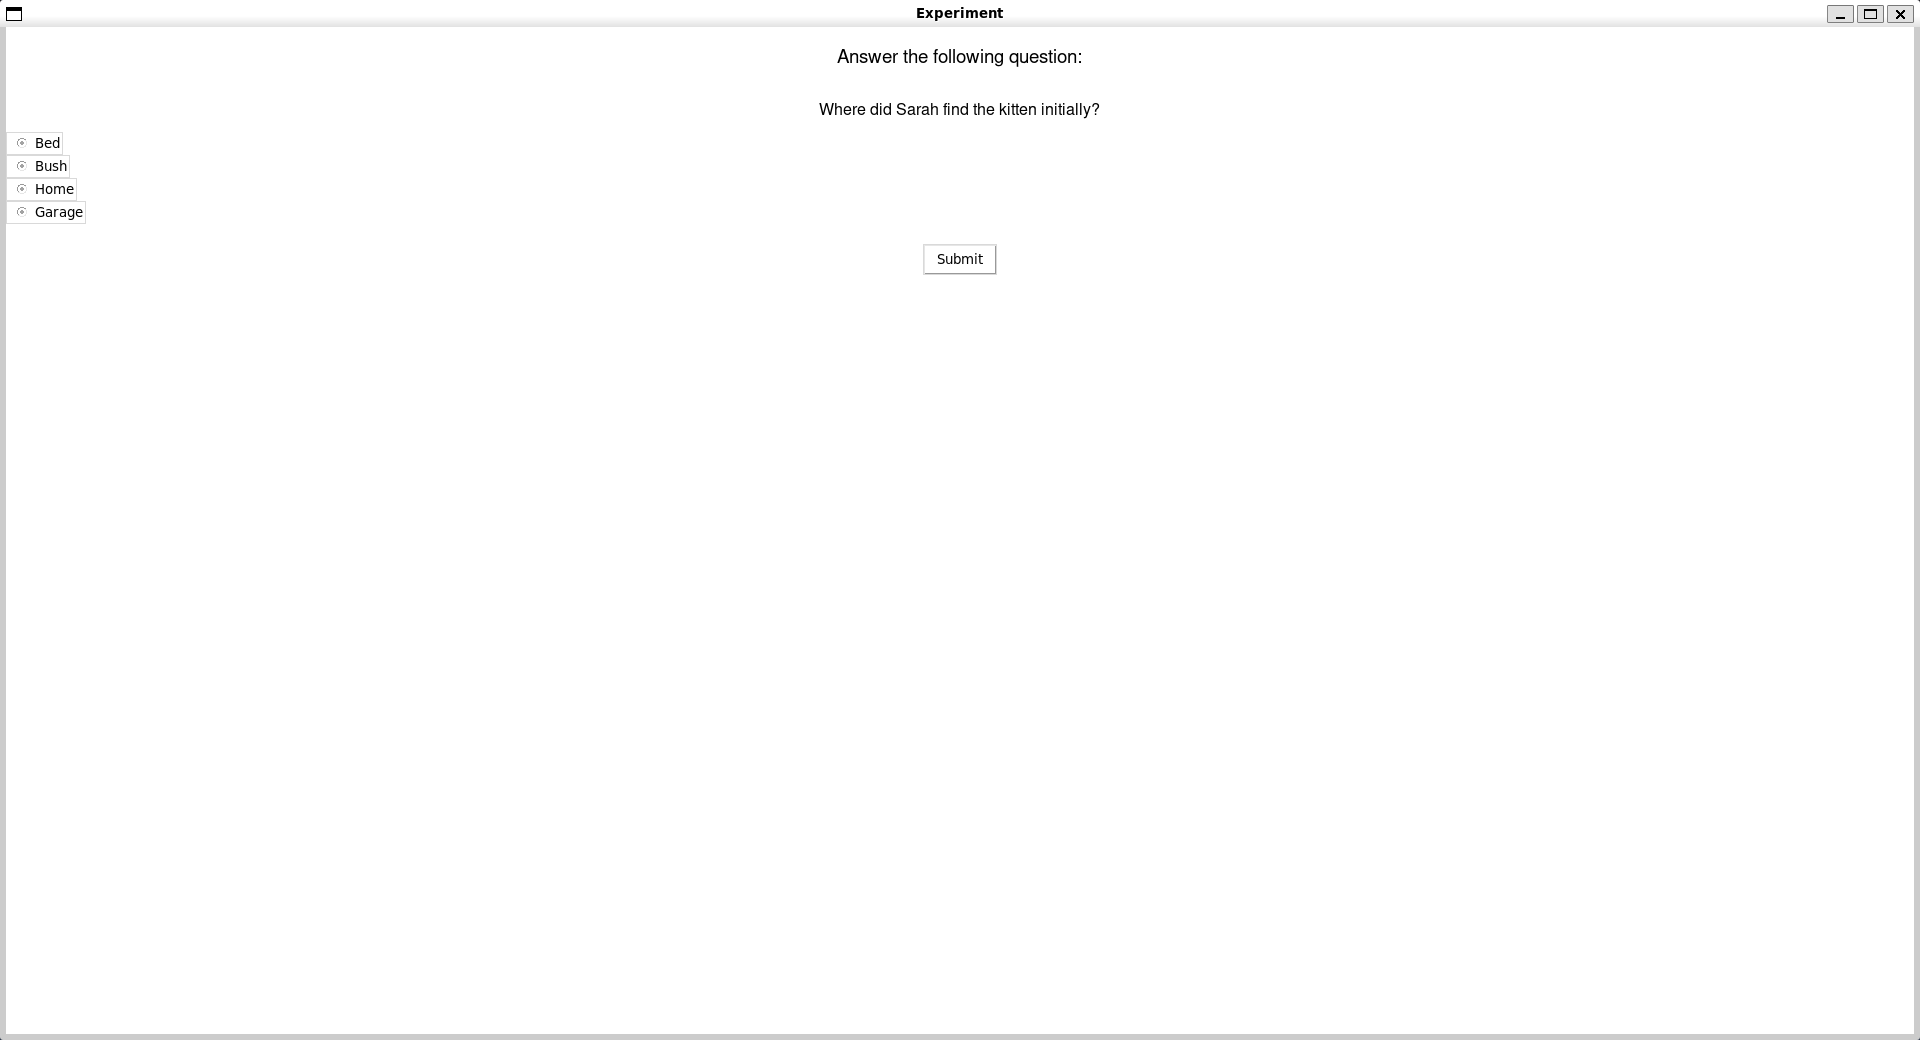
\includegraphics[width=\linewidth]{question-example.PNG}
  \caption{An example of a question asked.}
  \Description{"Where did Sarah find the kitten initially?," followed by the questions "Bed," "Bush," "Home," and "Garage."}
\end{figure}

\FloatBarrier

\subsection{Design.} 
The experiment followed a $1 \times 2$ within-subjects design. Participants were scored on a scale of 0 to 3 depending on the number of correct responses for each presentation method. Data collected from participant responses was analyzed to compare comprehension between the RSVP and static text conditions. The total number of trials was 4 participants $\times$ 1 story prompt $\times$ 2 presentation methods = 8.

\section{Results}
\subsection{Test Scores.}
The mean combined score for both sections is a score of 4.5 out of 6 or 75\%. The mean score for the RSVP quiz section was 1.75 out of 3 with a standard deviation of 0.75. The static reading method presented an increase of about 33.33\% with a mean score of 2.75 out of 3 and a standard deviation of 0.25.

Using these numbers, we can perform a t-test to determine statistical significance. The formula for a t-test is:
\begin{equation}
t = \frac{\bar{x}_1 - \bar{x}_2}{\sqrt{\frac{{s_1^2}}{{n_1}} + \frac{{s_2^2}}{{n_2}}}}
\end{equation}
where:
\begin{align*}
t & : \text{The calculated t-statistic} \\
\bar{x}_1, \bar{x}_2 & : \text{The means of the two groups} \\
s_1, s_2 & : \text{The standard deviations of the two groups} \\
n_1, n_2 & : \text{The sample sizes of the two groups}
\end{align*}
From this, we can calculate that the t-statistic is -2.53. Using the standard alpha value of 0.05, the critical t-value for a degrees of freedom equaling 6 is about 2.447 according to the table in Figure 6. Since the absolute value of -2.53 is greater-than 2.447, we reject the null and conclude there is indeed a statistically significant difference between the two methods.

\begin{figure}[htbp]
  \centering
  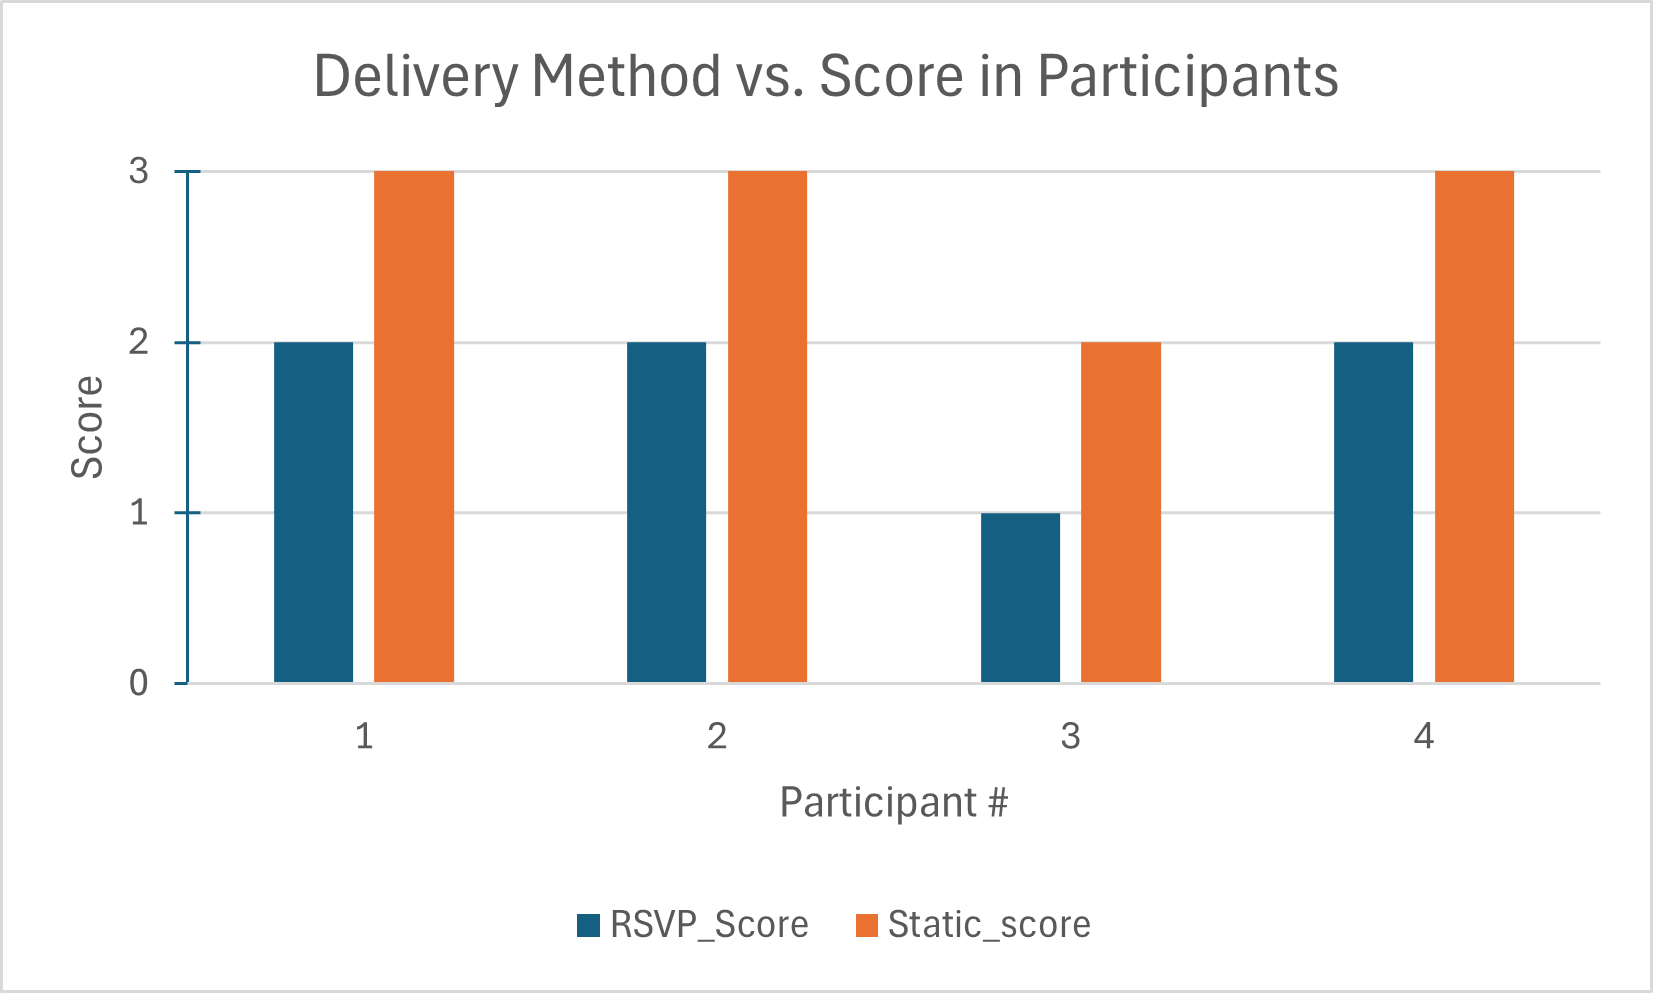
\includegraphics[width=\linewidth]{Delivery vs Score.png}
  \caption{Delivery method versus score.}
  \Description{"A bar graph plotting delivery method versus score."}
\end{figure}

\begin{figure}[htbp]
  \centering
  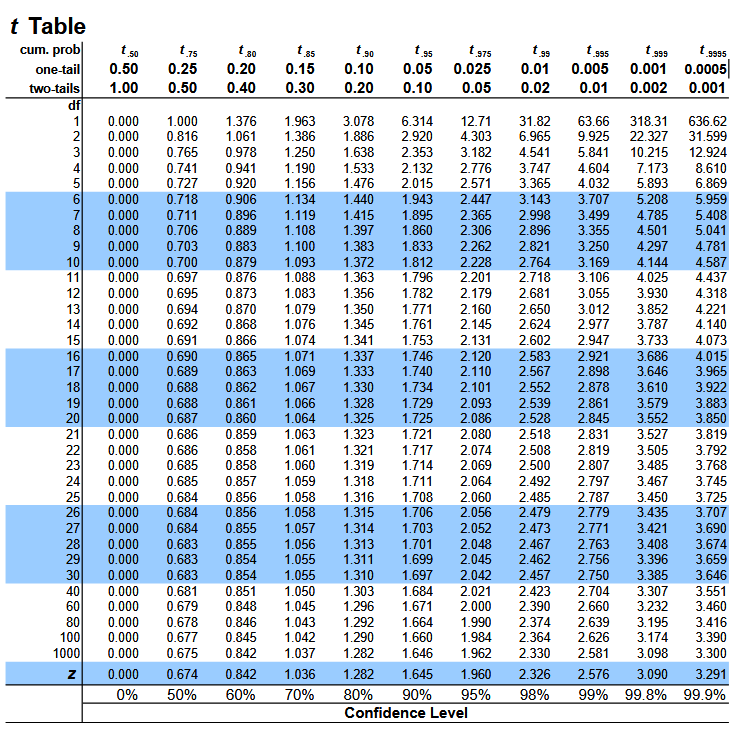
\includegraphics[width=\linewidth]{t-table.PNG}
  \caption{T-table used. Table taken from San Jose State University, via web. (\url{https://www.sjsu.edu/faculty/gerstman/StatPrimer/t-table.pdf}).}
  \Description{"A t-table for getting the critical t-value."}
\end{figure}

\FloatBarrier

\subsection{Participant Feedback.}
All participants reported no issues aside from one participant who reported that the white background caused some mild discomfort due to the brightness. Considering that both prompts were presented on the same background, it is safe to assume that this most likely had little-to-no bearing on the results.

\subsection{Discussion and Limitations.}
From the results gathered, there was indeed a difference found between the memory retention of participants when contrasting RSVP and static text delivery methods. Reader's memory retention tended to suffer when attempting to retrieve from a prompt read using RSVP. However, the sample size of four participants combined with the small question pool poses problems in terms of scalability.

\section{Conclusion and Future Work}
This study aimed to determine whether or not there posed a significant difference in memory retention for RSVP and static reading methods. What was found was that there was indeed a significant difference and that the static-based reading method was superior to the RSVP-based reading method, which falls in line with other similar studies conducted. However, due to the limitations of the methodology (see \S4.3), more study is needed. That being said, the results can provide a good basis for future investigations. And the feedback provided (see \S4.2) can allow for improvements on the methodology used by providing an option to lower screen brightness.

Interestingly enough, in terms of score, the question that had the most true responses for the RSVP section was the question asking what the main character's name was despite it only appearing once at the beginning of the prompt --- with three participants guessing it correctly as shown in Figure 7. Now, for the static section, the only question that got a wrong response was the one asking, "What were their initial emotions upon meeting?" Despite this question appearing at the beginning much like the previous question as well, it presented itself as the worst score-wise for the opposite section as shown in Figure 8, putting them on equal footing in terms of location. So, perhaps individuals have an easier time retaining names as opposed to other forms of information? A further study into this could be conducted by examining this phenomenon.

\begin{figure}[htbp]
  \centering
  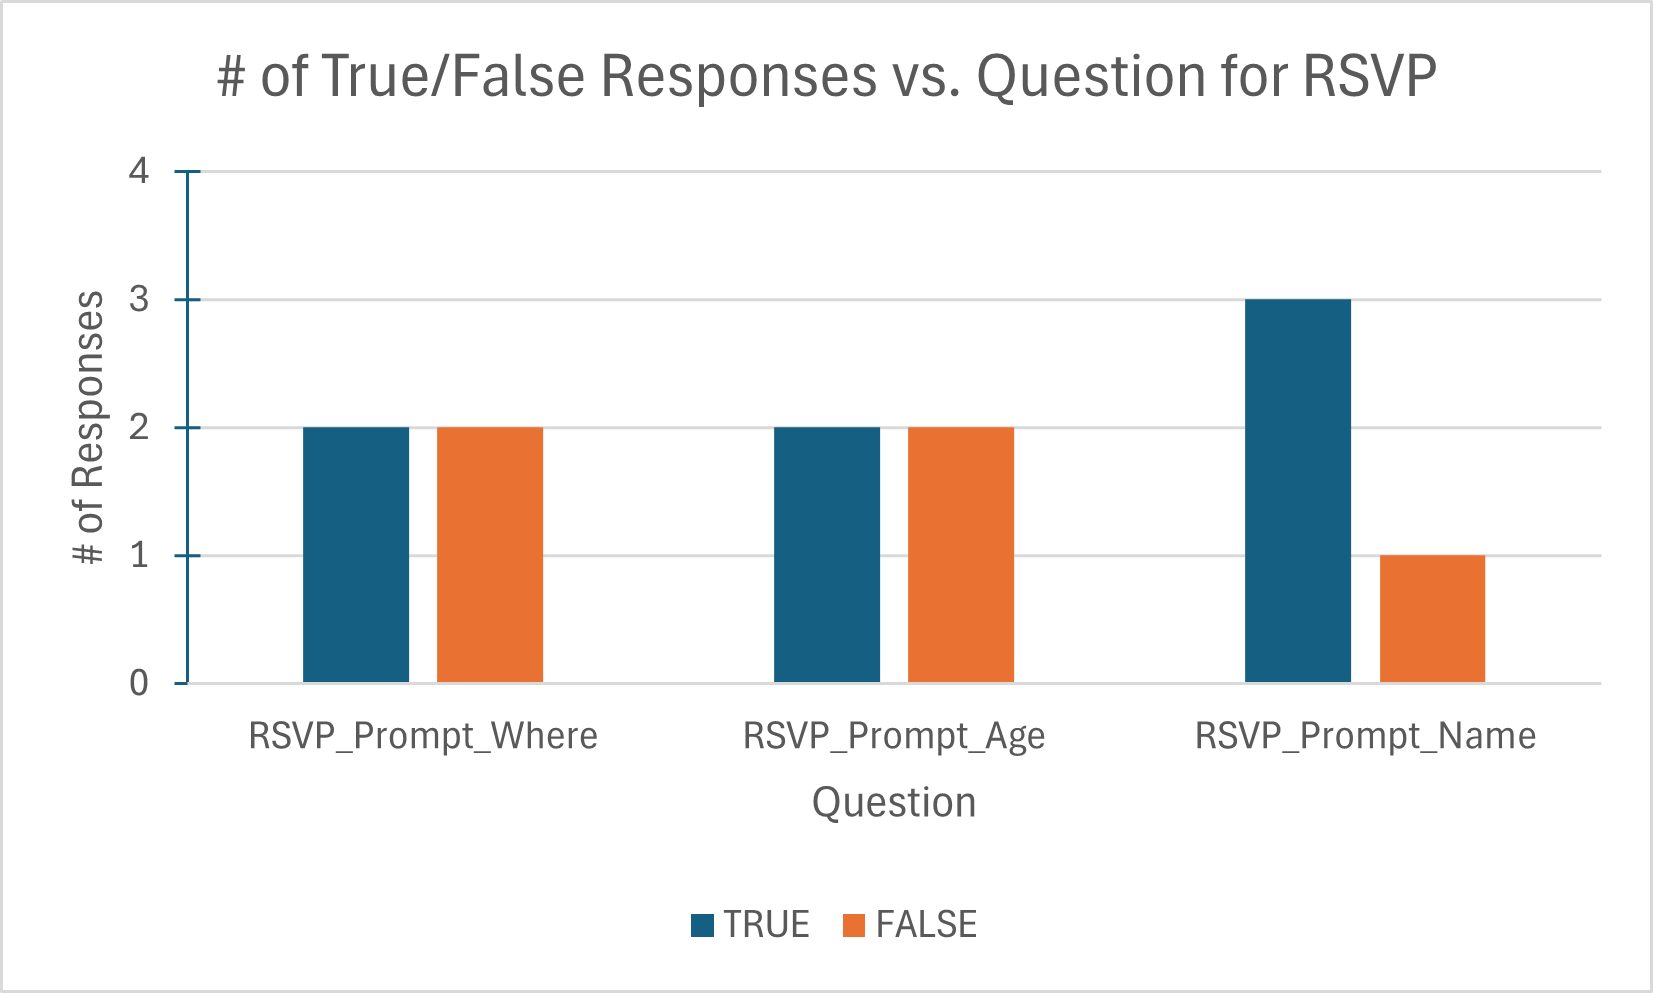
\includegraphics[scale=0.75]{Responses vs Question for RSVP.png}
  \caption{Responses versus score for the RSVP section.}
  \Description{"A bar graph plotting responses versus score for the RSVP section."}
\end{figure}

\begin{figure}[htbp]
  \centering
  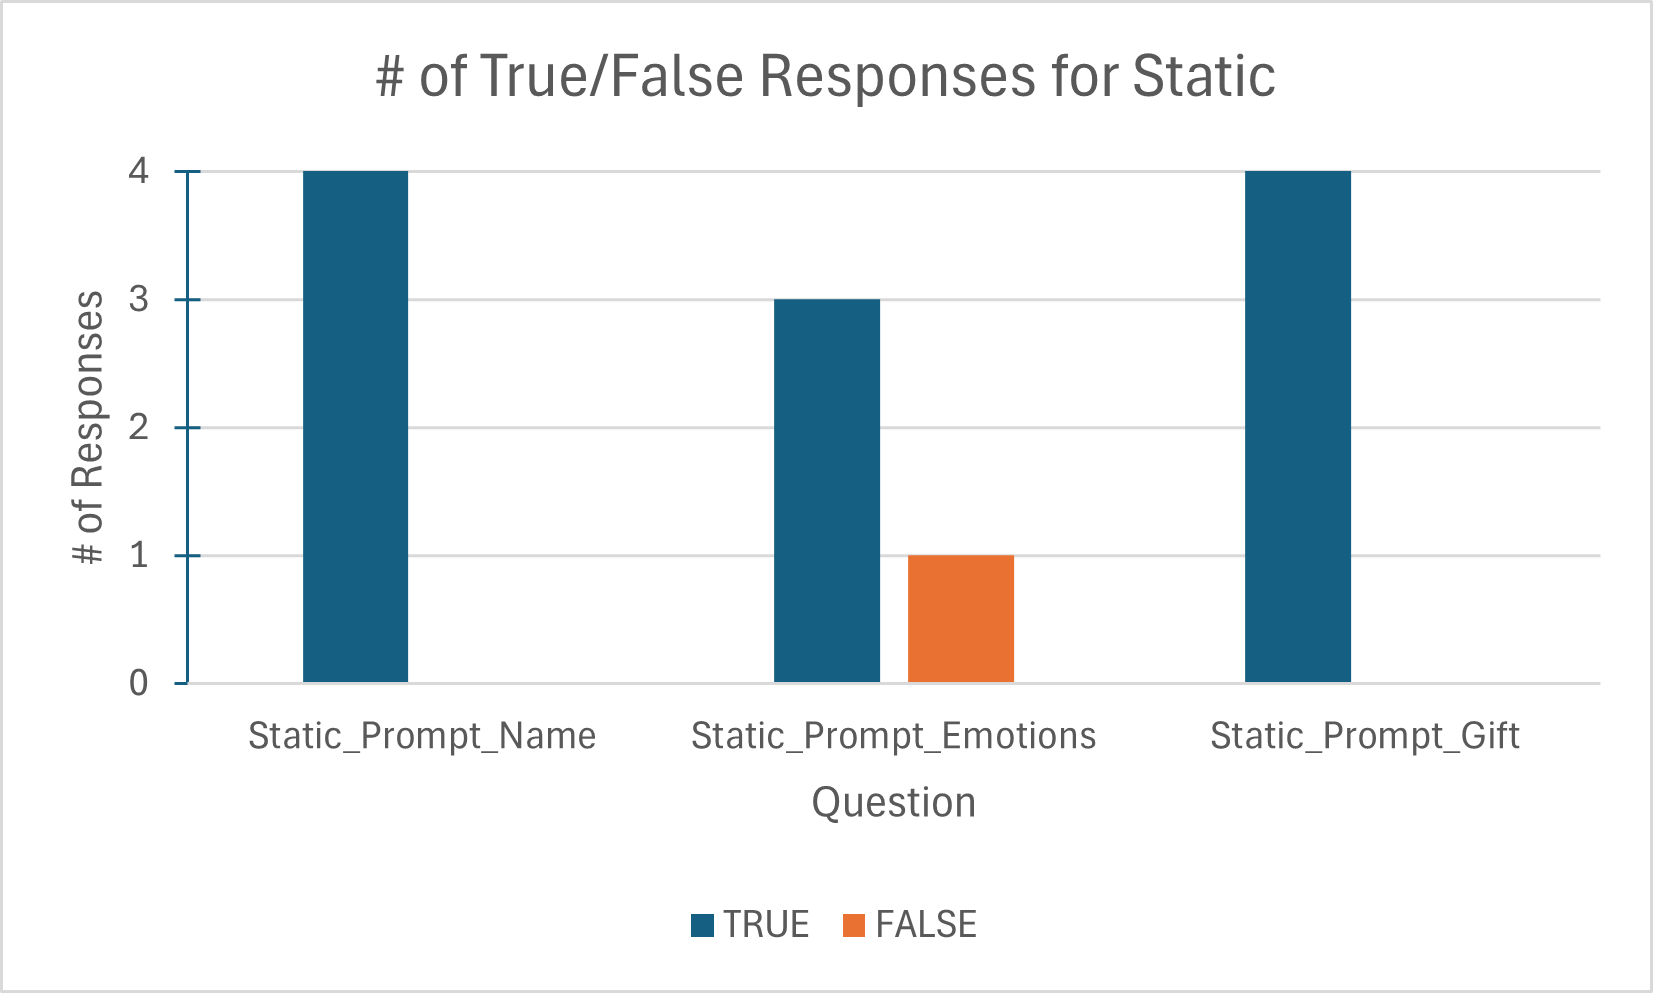
\includegraphics[scale=0.75]{Responses vs Question for Static.png}
  \caption{Responses versus score for the static section.}
  \Description{"A bar graph plotting responses versus score for the static section."}
\end{figure}

\FloatBarrier

\section{References}
\footnotesize
\begin{enumerate}
    \item Denis G. Pelli, Katharine A. Tillman, Jeremy Freeman, Michael Su, Tracey D. Berger, and Najib J. Majaj. "Crowding and eccentricity determine reading rate." Journal of Vision, 7(2):Oct, 2007. DOI: 10.1167/7.2.20. URL: https://doi.org/10.1167/7.2.20.
    \item Robert Spence. "Rapid, Serial and Visual: A Presentation Technique with Potential." Information Visualization, 1(1):Mar, 2002. DOI: 10.1057/palgrave.ivs.9500008. URL: https://doi.org/10.1057/palgrave.ivs.9500008.
    \item Gary S. Rubin and Kathleen Turano. "Reading without saccadic eye movements." Vision Research, 32(5):May, 1991, pages 895-902. DOI: 10.1016/0042-6989(92)90032-E. URL: https://doi.org/10.1016/0042-6989(92)90032-E.
    \item Rayner, K., Schotter, E. R., Masson, M. E. J., Potter, M. C., and Treiman, R. "So Much to Read, So Little Time: How Do We Read, and Can Speed Reading Help?" Psychological Science in the Public Interest, 17(1):Jan, 2016, pages 4-34. DOI: 10.1177/1529100615623267. URL: https://doi.org/10.1177/1529100615623267.
    \item Marc Brysbaert. "How many words do we read per minute? A review and meta-analysis of reading rate." Journal of Memory and Language, 109:Dec, 2019. DOI: 10.1016/j.jml.2019.104047. URL: https://doi.org/10.1016/j.jml.2019.104047.
    \item Richard Hall and Patrick Hanna. "The impact of web page text-background colour combinations on readability, retention, aesthetics and behavioural intention." Behaviour \& Information Technology, 23(3):Jun, 2004, pages 183-195. DOI: 10.1080/01449290410001669932. URL: https://doi.org/10.1080/01449290410001669932.
    \item Thomas Bohm. "Letter and symbol misrecognition in highly legible typefaces for general, children, dyslexic, visually impaired and ageing readers." Information Design Journal, Dec 2014. DOI: 10.1075/idj.21.1.05boh. URL: https://doi.org/10.1075/idj.21.1.05boh.
    \item Acklin D and Papesh MH. "Modern Speed-Reading Apps Do Not Foster Reading Comprehension." Am J Psychol, 2017, pages 183-199. DOI: 10.5406/amerjpsyc.130.2.0183. URL: https://doi.org/10.5406/amerjpsyc.130.2.0183.
    \item Chung STL and Bernard JB. "Bolder print does not increase reading speed in people with central vision loss." Vision Res, Dec 2018, pages 98-104. DOI: 10.1016/j.visres.2018.10.012. URL: http://doi.acm.org/10.1016/j.visres.2018.10.012.
    \item Fine EM and Peli E. "Benefits of rapid serial visual presentation (RSVP) over scrolled text vary with letter size." Optom Vis Sci, 75(3):Mar, 1998. DOI: 10.1097/00006324-199803000-00024. URL: https://doi.org/10.1097/00006324-199803000-00024.
\end{enumerate}


\end{document}
\endinput
%%
%% End of file `sample-manuscript.tex'.
